% L4a lecture companion deck.
% Mirrors the lecture notebook: graph definitions and measures; storage forms;
% the six-vertex worked example; graph families; traversal and shortest paths.
% Figure PDFs are built from standalone sources and Makefiles in ../figs.
\documentclass[aspectratio=169,11pt]{beamer}
\usepackage{vnslides}
\usepackage{tabularx}

\renewcommand{\vnlecturecode}{L4a}
\newcolumntype{Y}{>{\raggedright\arraybackslash}X}

\title{{\vnheavy L4a}: Graph and Tree Representations}
\subtitle{CHEME 5800 Cornell University}
\author{Copyright Jeffrey Varner 2026. All Rights Reserved}

\begin{document}

% ==== title ==================================================
\vntitlepage

% ==== objectives =============================================
\begin{frame}{Objectives for Today}
  Today we describe graph structure, calculate graph measures, and choose a
  storage form that matches the operation an algorithm performs.

  \vspace{0.9em}
  {\large\textbf{\ink{Today's concepts}}}
  \vspace{0.4em}
  \begin{itemize}\setlength{\itemsep}{0.7em}
    \item \hilite{Graph language and measures}: define walks, paths, cycles,
      connectivity, degree, and density.
    \item \hilite{Graph families}: recognize complete graphs, bipartite graphs,
      and trees from their defining properties.
    \item \hilite{Storage representations}: compare edge lists, adjacency
      matrices, and adjacency lists by storage and access cost.
  \end{itemize}

  \slidenote{Lecture:}{\href{https://github.com/varnerlab/CHEME-5800-CourseRepository-Fall-2026/blob/main/weeks/week-04/L4a/CHEME-5800-L4a-Lecture-GraphAndTreeRepresentations-Fall-2026.ipynb}{Graph and Tree Representations}}
\end{frame}

\begin{frame}{Lecture and Connected Exercises}
  \textbf{\ink{Lecture:}}
  \href{https://github.com/varnerlab/CHEME-5800-CourseRepository-Fall-2026/blob/main/weeks/week-04/L4a/CHEME-5800-L4a-Lecture-GraphAndTreeRepresentations-Fall-2026.ipynb}{Graph and Tree Representations}

  \vspace{1.0em}
  \textbf{\ink{Lab L4b:}}
  \href{https://github.com/varnerlab/CHEME-5800-CourseRepository-Fall-2026/blob/main/weeks/week-04/L4b/CHEME-5800-L4b-Lab-BreadthFirstAndDepthFirstSearch-Fall-2026.ipynb}{Breadth-First and Depth-First Search}

  Use an unweighted adjacency list to visit a directed graph with a queue or a stack.

  \vspace{1.0em}
  \textbf{\ink{Lecture L4c and lab L4d:}}
  \href{https://github.com/varnerlab/CHEME-5800-CourseRepository-Fall-2026/blob/main/weeks/week-04/L4c/CHEME-5800-L4c-Lecture-ShortestPathAlgorithms-Fall-2026.ipynb}{Shortest-Path Algorithms}

  Retain edge weights and find minimum-cost routes through a process network.
\end{frame}

% ==== simple graphs ==========================================
\begin{frame}{Simple Graphs}
  A simple graph $\mathcal G=(\mathcal V,\mathcal E)$ consists of a set of vertices
  $\mathcal V$ and a set of edges $\mathcal E$.

  \vspace{0.8em}
  \begin{itemize}\setlength{\itemsep}{0.8em}
    \item In an \hilite{undirected graph}, an edge $\{u,v\}$ is an unordered
      pair of distinct vertices and may be followed either way.
    \item In a \hilite{directed graph}, an edge $(u,v)$ is an ordered pair.
      It points from $u$ to $v$, and $(v,u)$ is a different edge.
    \item The word \hilite{simple} rules out self-loops and repeated parallel edges.
    \item An edge may carry a weight such as distance, capacity, time, or cost.
  \end{itemize}

  \slidenote{Modeling decision:}{direction records which transitions are feasible; weight records a quantity associated with an edge.}
\end{frame}

\begin{frame}{Direction Changes Which Routes Are Feasible}
  \begin{center}
    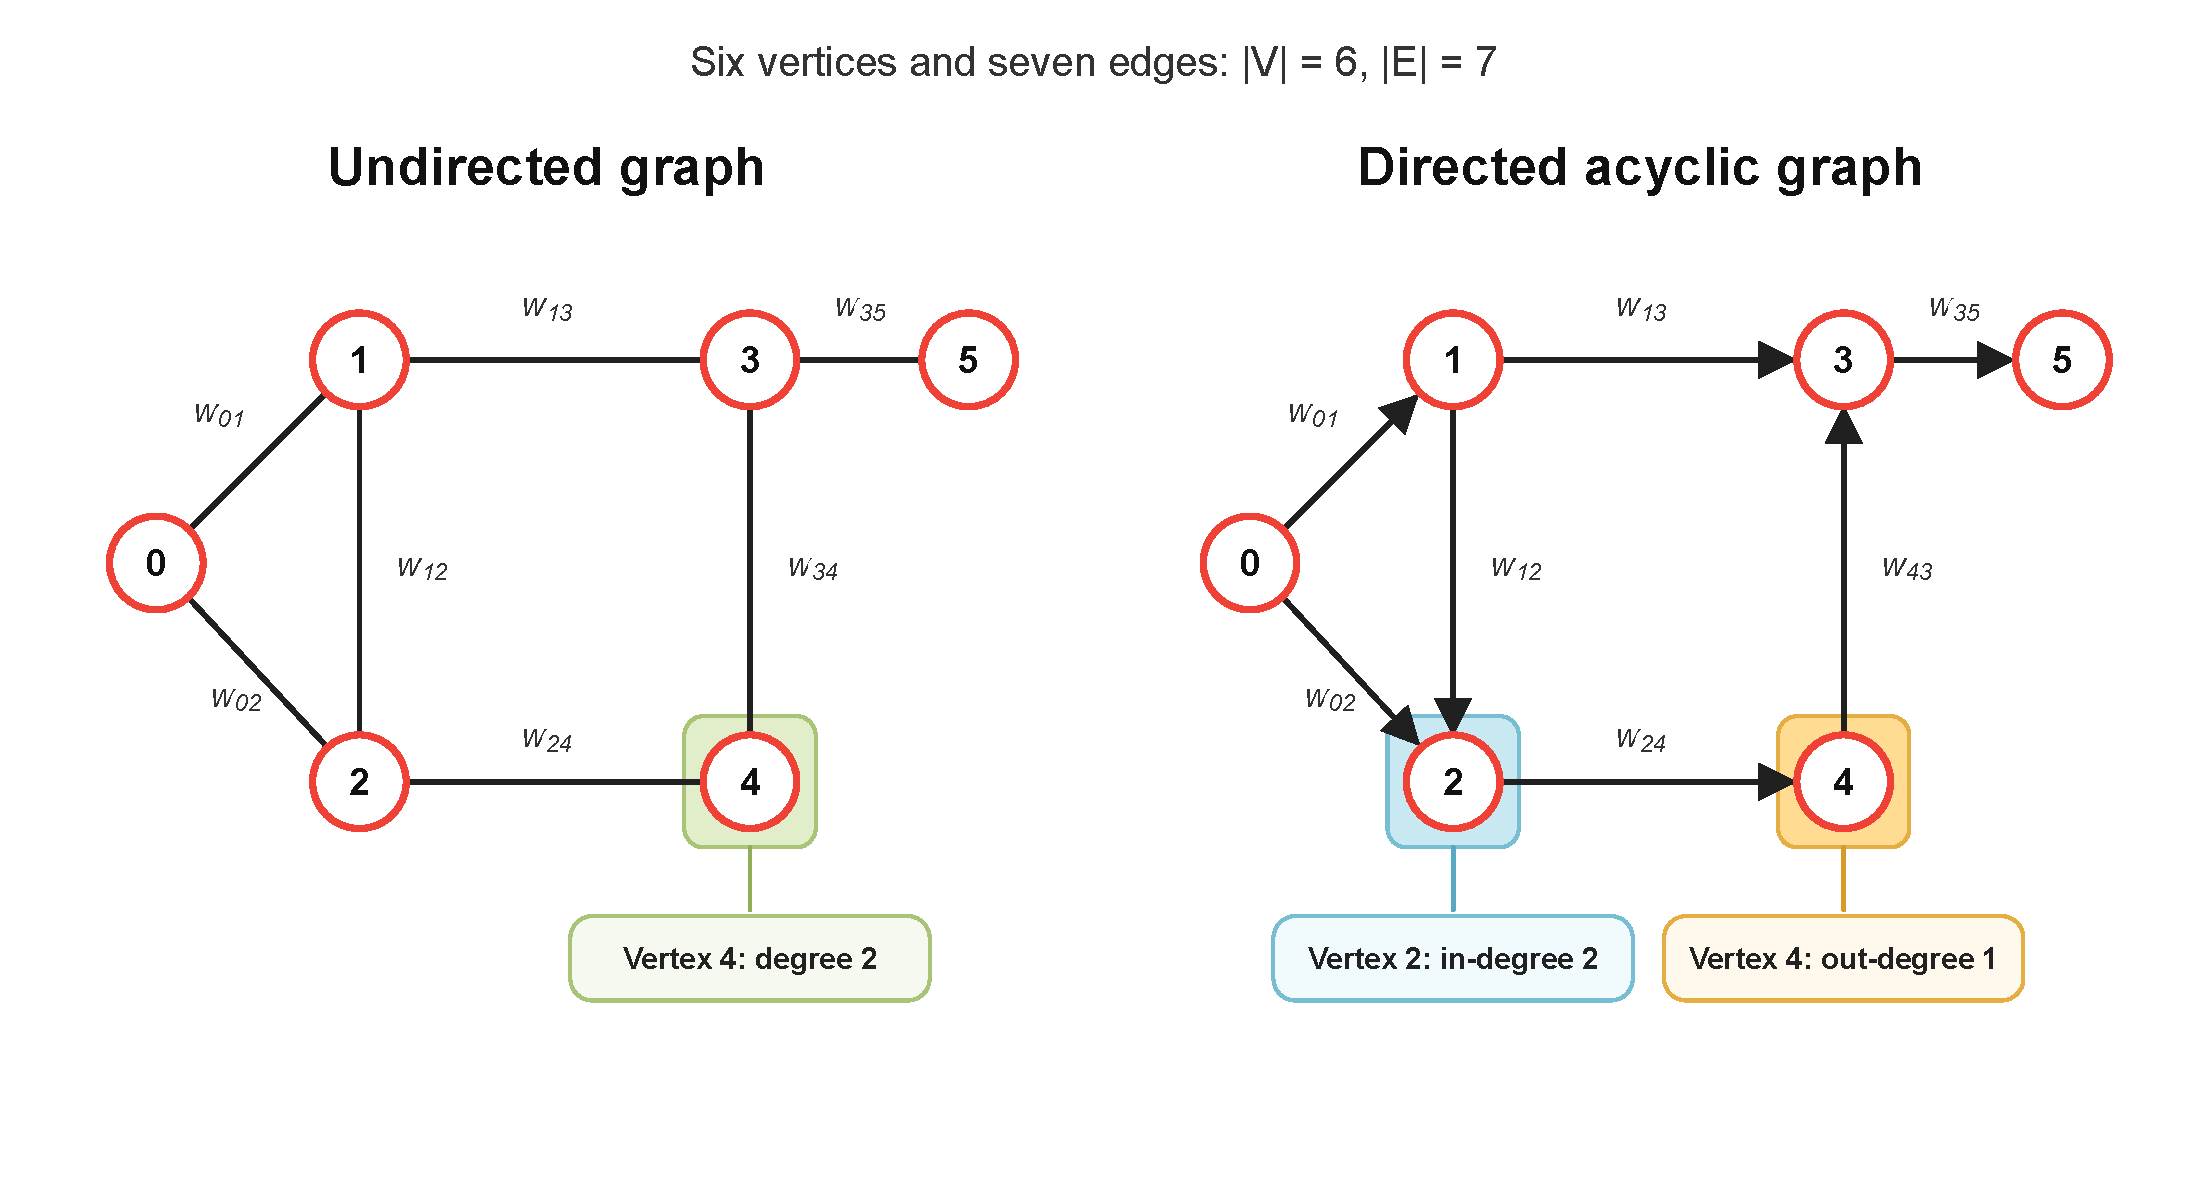
\includegraphics[height=0.80\textheight,keepaspectratio]{assets/Fig-General-Graph-Schematic.pdf}
  \end{center}

  \vspace{-0.2em}
  The undirected drawing allows travel across an edge in either direction. The
  directed drawing allows only the arrow direction, even when the endpoints match.
\end{frame}

\begin{frame}{Walks, Paths, and Cycles}
  Let $v_0,v_1,\ldots,v_k$ be a sequence of vertices.

  \vspace{0.8em}
  \begin{itemize}\setlength{\itemsep}{0.85em}
    \item A \hilite{walk} follows an edge between every consecutive pair. A
      directed walk must follow every source-to-target direction.
    \item A \hilite{path} is a walk with no repeated vertices.
    \item A \hilite{cycle} is a closed walk with at least one edge that repeats
      no edge and no vertex except $v_0=v_k$.
  \end{itemize}

  \vspace{0.5em}
  A path never revisits a vertex. A cycle returns to its starting vertex.
\end{frame}

\begin{frame}{Connectivity Depends on Direction}
  Connectivity asks whether paths join the vertices.

  \vspace{0.8em}
  \begin{itemize}\setlength{\itemsep}{0.85em}
    \item An undirected graph is \hilite{connected} when a path joins every pair
      of vertices.
    \item A directed graph is \hilite{weakly connected} when ignoring edge
      directions produces a connected undirected graph.
    \item A directed graph is \hilite{strongly connected} when every ordered pair
      $(u,v)$ is joined by a directed path from $u$ to $v$.
  \end{itemize}

  \vspace{0.5em}
  In the figure, vertex 0 can reach vertex 5, but vertex 5 has no outgoing edge.
  The directed graph is weakly but not strongly connected. It has no directed
  cycles, so it is a \hilite{directed acyclic graph}.
\end{frame}

% ==== graph measures =========================================
\begin{frame}{Directed Degree Has Two Parts}
  Count the edges touching vertex 4. Only its incident edges are shown.

  \vspace{1.0em}
  \begin{columns}[T,onlytextwidth]
    \begin{column}{0.47\textwidth}
      \centering
      {\large\textbf{\ink{Undirected}}}

      \vspace{1.2em}
      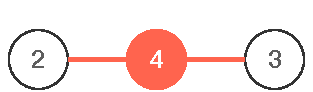
\includegraphics{../figs/Fig-Degree-Undirected/Fig-Degree-Undirected.pdf}

      \vspace{0.8em}
      Two edges touch vertex 4.
      \[
        \deg(v_4)=2
      \]
    \end{column}
    \begin{column}{0.47\textwidth}
      \centering
      {\large\textbf{\ink{Directed}}}

      \vspace{1.2em}
      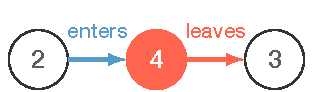
\includegraphics{../figs/Fig-Degree-Directed/Fig-Degree-Directed.pdf}

      \vspace{0.8em}
      One edge enters; one leaves.
      \[
        \textcolor{vnslidelink}{\deg^{\mathrm{in}}(v_4)=1},\qquad
        \textcolor{vnaccent}{\deg^{\mathrm{out}}(v_4)=1}
      \]
    \end{column}
  \end{columns}

  \vspace{0.7em}
  \begin{center}
    Total degree: $\deg(v_4)=\deg^{\mathrm{in}}(v_4)+\deg^{\mathrm{out}}(v_4)=2$.
  \end{center}
\end{frame}

\begin{frame}{Degree Counts Recover the Edge Count}
  Let $n=|\mathcal V|$ and $m=|\mathcal E|$.
  In an undirected graph, summing degrees counts both endpoints of every edge:
  \[
    \underbrace{\sum_{v_i\in\mathcal V}\deg(v_i)}_{\text{all incident ends}}=2m.
  \]

  In a directed graph, each edge contributes once to each directional sum:
  \[
    \underbrace{\sum_{v_i\in\mathcal V}\deg^{\mathrm{in}}(v_i)}_{\text{all targets}}
    =
    \underbrace{\sum_{v_i\in\mathcal V}\deg^{\mathrm{out}}(v_i)}_{\text{all sources}}
    =m.
  \]

  These \hilite{handshaking identities} are useful consistency checks for graph data.
\end{frame}

\begin{frame}{Average Degree Lies Between the Extremes}
  For an undirected graph with $n\geq1$, let $\delta(\mathcal G)$ and
  $\Delta(\mathcal G)$ be its minimum and maximum degrees.
  The average degree is given by:
  \[
    \underbrace{\bar d(\mathcal G)=\frac{1}{n}
      \sum_{v_i\in\mathcal V}\deg(v_i)=\frac{2m}{n}}_{\text{average degree}}.
  \]
  It is bounded by:
  \[
    \delta(\mathcal G)\leq\bar d(\mathcal G)\leq\Delta(\mathcal G).
  \]

  An undirected graph is \hilite{regular of degree $r$} when every vertex has
  degree $r$. Then $\delta=\bar d=\Delta=r$.
\end{frame}

\begin{frame}{Density Measures the Fraction of Possible Edges}
  A simple loop-free graph on $n\geq2$ vertices has maximum edge count:
  \[
    |\mathcal E|_{\max}=
    \begin{cases}
      n(n-1)/2, & \text{undirected},\\
      n(n-1), & \text{directed}.
    \end{cases}
  \]
  The density is the observed fraction of that maximum:
  \[
    \underbrace{\rho(\mathcal G)=\frac{|\mathcal E|}{|\mathcal E|_{\max}}}_{\text{graph density}},
    \qquad 0\leq\rho(\mathcal G)\leq1.
  \]

  Density near one is \hilite{dense}; density near zero is \hilite{sparse}.
  This lecture sets $\rho(\mathcal G)=0$ when $n<2$.
\end{frame}

\begin{frame}{Four Measures Describe Graph Arrangement}
  For an undirected graph, counts can be supplemented by:

  \vspace{0.7em}
  \begin{itemize}\setlength{\itemsep}{0.65em}
    \item \hilite{Diameter $\operatorname{diam}(\mathcal G)$}: the largest
      shortest-path distance in a connected graph, measured in edges.
    \item \hilite{Clique number $\omega(\mathcal G)$}: the largest number of
      vertices that are all pairwise adjacent.
    \item \hilite{Chromatic number $\chi(\mathcal G)$}: the fewest colors that
      place different colors on adjacent vertices.
    \item \hilite{Independence number $\alpha(\mathcal G)$}: the largest number
      of vertices with no edge between any selected pair.
  \end{itemize}

  \slidenote{Computational consequence:}{these measures require edge lookups and neighbor iteration; vertex and edge counts alone are insufficient.}
\end{frame}

\begin{frame}{Path and Star Graphs}
  Both graphs have $n=6$ vertices and $n-1=5$ edges.

  \vspace{0.7em}
  \begin{columns}[T,onlytextwidth]
    \begin{column}{0.47\textwidth}
      \centering
      {\large\textbf{\ink{Path graph}}}

      \vspace{0.4em}
      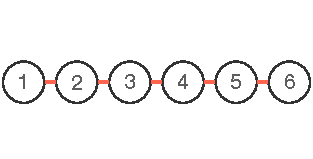
\includegraphics{../figs/Fig-Path-Graph/Fig-Path-Graph.pdf}

      Maximum degree: $\Delta=2$\par
      \vspace{0.3em}
      Diameter: $n-1=\hilite{5}$ edges
    \end{column}
    \begin{column}{0.47\textwidth}
      \centering
      {\large\textbf{\ink{Star graph}}}

      \vspace{0.4em}
      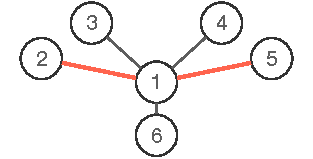
\includegraphics{../figs/Fig-Star-Graph/Fig-Star-Graph.pdf}

      Maximum degree: $\Delta=n-1=5$\par
      \vspace{0.3em}
      Diameter: $\hilite{2}$ edges
    \end{column}
  \end{columns}

  \vspace{1.0em}
  The \hilite{highlighted route} joins a most distant pair of vertices.
\end{frame}

% ==== storage forms ==========================================
\transitionframe{The graph is a mathematical object. \hilite{Its representation
determines what an algorithm can access efficiently.}}

\begin{frame}{Three Forms Store the Same Graph}
  Let $n=|\mathcal V|$ and $m=|\mathcal E|$.

  \vspace{0.8em}
  \begin{itemize}\setlength{\itemsep}{0.85em}
    \item An \hilite{edge list} stores one source-target-weight record per edge.
    \item An \hilite{adjacency matrix} stores one entry for every ordered pair
      of vertices.
    \item An \hilite{adjacency list} stores one outgoing-neighbor collection per vertex.
  \end{itemize}

  \vspace{0.5em}
  Each form can describe the same graph, provided its vertex set is retained.
  The representation affects edge lookup and neighbor iteration.
\end{frame}

\begin{frame}{Edge Lists Store One Record per Edge}
  An edge list stores each edge's endpoints and, when present, its weight.

  \vspace{0.8em}
  \begin{itemize}\setlength{\itemsep}{0.8em}
    \item Edge records require $\Theta(m)$ storage. An explicit vertex set adds
      $\Theta(n)$, giving $\Theta(n+m)$ overall.
    \item Isolated vertices do not appear in edge records and must be stored separately.
    \item Without an index, finding an edge or collecting a vertex's neighbors
      takes $\Theta(1+m)$ time in the worst case.
  \end{itemize}

  \vspace{0.5em}
  Edge lists suit reading, writing, and scanning the complete edge collection.
\end{frame}

\begin{frame}{Adjacency Matrices Reserve Every Vertex Pair}
  For vertex order $v_1,\ldots,v_n$, an unweighted adjacency matrix has entries:
  \[
    a_{ij}=\begin{cases}
      1, & \text{an edge joins }v_i\text{ to }v_j,\\
      0, & \text{otherwise}.
    \end{cases}
  \]
  In a weighted matrix, an existing edge's entry stores its weight $w_{ij}$.

  \vspace{0.5em}
  \begin{itemize}\setlength{\itemsep}{0.55em}
    \item Storage is $\Theta(n^2)$ and one edge lookup is $\Theta(1)$.
    \item Listing neighbors of $v_i$ scans row $i$ in $\Theta(n)$ time.
    \item An undirected matrix is symmetric; a directed matrix need not be.
  \end{itemize}

  \slidenote{Zero weights:}{zero can mark a missing edge only when it is not a valid edge weight; otherwise use a separate marker.}
\end{frame}

\begin{frame}{Adjacency Lists Store Neighbors}
  An adjacency list stores one collection of outgoing neighbors for each source.

  \vspace{0.7em}
  \begin{itemize}\setlength{\itemsep}{0.7em}
    \item Unweighted form: \texttt{source => [target, ...]}.
    \item Weighted form: \texttt{source => [(target, weight), ...]}.
    \item Storage is $\Theta(n+m)$ for a directed graph.
    \item Accessing a source's dictionary entry is expected $\Theta(1)$;
      iterating over its out-neighbors costs
      $\Theta(1+\deg^{\mathrm{out}}(v_i))$.
  \end{itemize}

  In an undirected list, each edge appears in both endpoint lists. The exact
  count is $n+2m$ vertex and neighbor records, which remains $\Theta(n+m)$.
\end{frame}

\begin{frame}{Pair Lists with an Edge-Weight Map}
  A flat dictionary can map a known endpoint pair directly to a weight:
  \[
    (u,v)\longmapsto w(u,v).
  \]

  \vspace{0.6em}
  \begin{itemize}\setlength{\itemsep}{0.75em}
    \item Expected lookup for a known $(u,v)$ is $\Theta(1)$.
    \item Finding all neighbors of $u$ still requires scanning $m$ entries.
    \item Pairing the map with an unweighted adjacency list gives fast direct
      weight lookup and fast neighbor iteration.
  \end{itemize}

  \slidenote{Design principle:}{one graph object may maintain more than one representation when its algorithms require different access patterns.}
\end{frame}

\begin{frame}{Storage and Access Costs}
  Let $d_u=\deg^{\mathrm{out}}(u)$. For a directed graph:

  \vspace{0.6em}
  \renewcommand{\arraystretch}{1.38}
  \begin{tabularx}{\textwidth}{>{\vnmedium}Xlll}
    \toprule
    Representation & Storage & Find $(u,v)$ & List neighbors \\
    \midrule
    Edge list + vertex set & $\Theta(n+m)$ & $\Theta(1+m)$ & $\Theta(1+m)$ \\
    Adjacency matrix & $\Theta(n^2)$ & $\Theta(1)$ & $\Theta(n)$ \\
    Adjacency list & $\Theta(n+m)$ & $\Theta(1+d_u)$ & $\Theta(1+d_u)$ \\
    \bottomrule
  \end{tabularx}

  \vspace{0.8em}
  Edge searches use worst-case scan lengths; dictionary access is expected
  constant time. The added 1 includes the work needed for an empty list.

  \slidenote{Weight lookup:}{a separate edge-weight map provides expected $\Theta(1)$ access to a known vertex pair.}
\end{frame}

\begin{frame}{Choose the Representation from the Operation}
  \textbf{\ink{Does the edge $(u,v)$ exist?}}\quad\hilite{Adjacency matrix}

  Read $A_{uv}$ directly in $\Theta(1)$ time. Repeated edge lookups favor a
  matrix when its $\Theta(n^2)$ storage is affordable, especially for dense graphs.

  \vspace{1.0em}
  \textbf{\ink{Which vertices are neighbors of $u$?}}\quad\hilite{Adjacency list}

  Scan the $d_u$ neighbors of $u$ instead of all $n$ matrix entries.
  For a sparse graph, this reduces neighbor-search work and uses
  $\Theta(n+m)$ storage.

  \vspace{1.0em}
  \textbf{\ink{How do we process every edge?}}\quad\hilite{Edge list}

  Read, write, or sort the edges as records. A full scan takes $\Theta(m)$
  time, but finding one vertex's neighbors also requires scanning the list.

  \vspace{0.8em}
  Balance the work done most often against the storage available.
\end{frame}

% ==== worked example =========================================
\begin{frame}{Worked Example: A Six-Vertex Directed Graph}
  The file \texttt{SimpleGraph.txt} contains seven weighted edge records:

  \vspace{0.6em}
  \begin{columns}[T,onlytextwidth]
    \begin{column}{0.33\textwidth}
      \small
      \begin{tabular}{rrr}
        \toprule
        source & target & weight \\
        \midrule
        1&2&10\\ 1&3&100\\ 2&3&2\\ 2&4&100\\
        3&5&6\\ 4&6&1\\ 5&4&1\\
        \bottomrule
      \end{tabular}
    \end{column}
    \begin{column}{0.63\textwidth}
      \begin{center}
      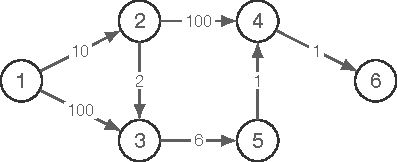
\includegraphics{../figs/Fig-Six-Vertex-Directed-Graph/Fig-Six-Vertex-Directed-Graph.pdf}
      \end{center}
    \end{column}
  \end{columns}

  \slidenote{Notebook functions:}{\texttt{read\_weighted\_edges}, \texttt{adjacency\_list}, and \texttt{adjacency\_matrix}.}
\end{frame}

\begin{frame}{The Same Edges Become a List or a Matrix}
  \begin{columns}[T,onlytextwidth]
    \begin{column}{0.39\textwidth}
      {\large\textbf{\ink{Outgoing adjacency list}}}
      \vspace{0.6em}

      \begin{tabular}{c@{\ $\longrightarrow$\ }l}
        1 & $[2,3]$\\
        2 & $[3,4]$\\
        3 & $[5]$\\
        4 & $[6]$\\
        5 & $[4]$\\
        6 & $[\,]$\\
      \end{tabular}

      \vspace{0.8em}
      This lecture's helper stores targets only; the original edge records retain the weights.
    \end{column}
    \begin{column}{0.57\textwidth}
      {\large\textbf{\ink{Weighted adjacency matrix}}}
      \vspace{0.4em}
      \[
      \begin{array}{c|rrrrrr}
          &1&2&3&4&5&6\\\hline
        1&0&10&100&0&0&0\\
        2&0&0&2&100&0&0\\
        3&0&0&0&0&6&0\\
        4&0&0&0&0&0&1\\
        5&0&0&0&1&0&0\\
        6&0&0&0&0&0&0
      \end{array}
      \]
    \end{column}
  \end{columns}
\end{frame}

\begin{frame}{Vertex Labels and Matrix Indices}
  Relabel the same six vertices as $10,20,30,40,50,60$; keep all edges and weights.
  Choose $\texttt{vertex\_order}=[10,20,30,40,50,60]$.

  \vspace{0.8em}
  \begin{columns}[T,onlytextwidth]
    \begin{column}{0.38\textwidth}
      \centering
      \textbf{\ink{Index-to-vertex mapping}}

      \vspace{0.4em}
      \renewcommand{\arraystretch}{1.0}
      \begin{tabular}{cc}
        \toprule
        Index $i$ & Vertex label \\
        \midrule
        \hilite{1} & \hilite{10} \\
        2 & 20 \\
        \hilite{3} & \hilite{30} \\
        4 & 40 \\
        5 & 50 \\
        6 & 60 \\
        \bottomrule
      \end{tabular}
    \end{column}
    \begin{column}{0.58\textwidth}
      \centering
      \textbf{\ink{Weighted adjacency matrix}}
      \[
        A=\begin{array}{c|rrrrrr}
           &1&2&\hilite{3}&4&5&6\\\hline
          \hilite{1}&0&10&\hilite{100}&0&0&0\\
          2&0&0&2&100&0&0\\
          3&0&0&0&0&6&0\\
          4&0&0&0&0&0&1\\
          5&0&0&0&1&0&0\\
          6&0&0&0&0&0&0
        \end{array}
      \]
    \end{column}
  \end{columns}

  \vspace{0.8em}
  $\hilite{A_{1,3}=100}$ records the edge $\hilite{10\to30}$ with weight 100.
\end{frame}

\begin{frame}{Graph Storage: Counts and Growth}
  Our directed example has $n=6$, $m=7$, and
  $\rho=7/[6(6-1)]=7/30$.

  \vspace{0.7em}
  \renewcommand{\arraystretch}{1.25}
  \begin{tabularx}{\textwidth}{Xll}
    \toprule
    \textbf{Graph} & \textbf{Adjacency matrix} & \textbf{Adjacency list} \\
    \midrule
    Six-vertex example & $n^2=36$ entries & $n+m=13$ items \\
    Sparse: $m=10n$ & $\Theta(n^2)$ & $\Theta(n+10n)=\Theta(n)$ \\
    Dense: $m=\Theta(n^2)$ & $\Theta(n^2)$ & $\Theta(n^2)$ \\
    \bottomrule
  \end{tabularx}

  \vspace{0.8em}
  The matrix reserves space for absent edges. The example's list stores
  6 vertex collections and 7 neighbor entries.

  \vspace{0.6em}
  Big Theta describes storage growth as well as running time. With 10 outgoing
  edges per vertex, doubling $n$ approximately doubles list storage but quadruples
  matrix storage.
\end{frame}

% ==== graph families =========================================
\transitionframe{Three graph families turn structural definitions into
\hilite{recognition tests, edge counts, and storage requirements.}}

\begin{frame}{Complete Graphs Use Every Possible Edge}
  A complete graph $K_n$ is a simple undirected graph with an edge between every
  pair of distinct vertices.

  \vspace{0.25em}
  \begin{center}
    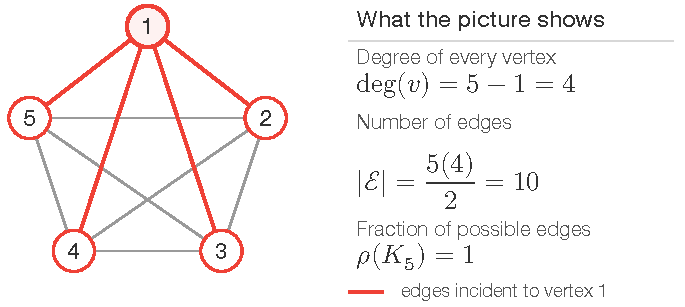
\includegraphics[height=0.66\textheight]{../figs/Fig-Complete-Graph-Schematic/Fig-Complete-Graph-Schematic-panel.pdf}
  \end{center}
\end{frame}

\begin{frame}{Complete-Graph Measures Follow Directly}
  For $n\geq2$, every possible edge is present:
  \[
    |\mathcal E|=\binom n2=\frac{n(n-1)}{2},\qquad
    \deg(v_i)=n-1.
  \]
  Consequently:
  \[
    \rho(K_n)=1,\qquad \operatorname{diam}(K_n)=1,
  \]
  \[
    \omega(K_n)=\chi(K_n)=n,\qquad \alpha(K_n)=1.
  \]

  \href{https://nrich.maths.org/articles/tournament-scheduling}{Round-robin schedules}
  have the edge pattern of $K_n$.
  \href{https://www.math.uwaterloo.ca/tsp/college/index.html}{Traveling-salesman models}
  use a weighted $K_n$ when every city pair has a symmetric travel cost.

  \slidenote{Storage:}{since $|\mathcal E|=\Theta(n^2)$, both matrices and adjacency lists require $\Theta(n^2)$ storage.}
\end{frame}

\begin{frame}{Bipartite Graphs Split Vertices into Two Groups}
  A graph is bipartite when
  $\mathcal V=\mathcal V_1\mathbin{\dot\cup}\mathcal V_2$ and every edge has
  one endpoint in each group.

  \vspace{0.15em}
  \begin{center}
    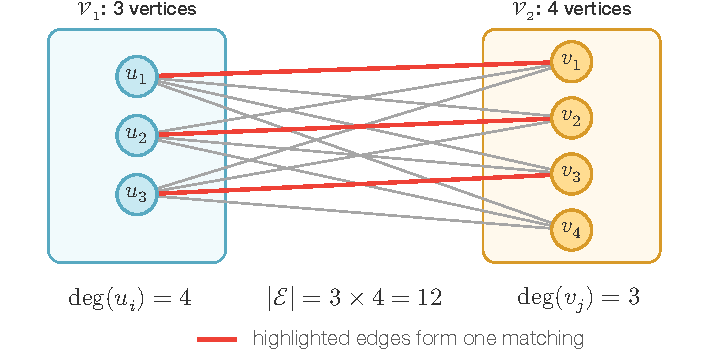
\includegraphics[width=0.94\textwidth,height=0.70\textheight,keepaspectratio]{../figs/Fig-Bipartite-Graph-Schematic/Fig-Bipartite-Graph-Schematic-panel.pdf}
  \end{center}
\end{frame}

\begin{frame}{Complete Bipartite Graphs}
  A complete bipartite graph $K_{m,n}$ includes every edge between its two
  groups and no edge within a group.

  \vspace{0.5em}
  \begin{columns}[T,onlytextwidth]
    \begin{column}{0.45\textwidth}
      \centering
      \textbf{\ink{The graph $K_{3,4}$}}

      \vspace{0.4em}
      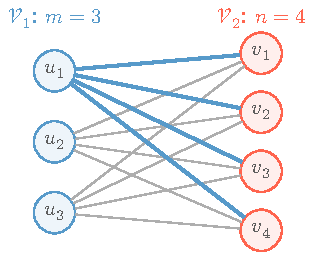
\includegraphics{../figs/Fig-Complete-Bipartite-Graph/Fig-Complete-Bipartite-Graph.pdf}
    \end{column}
    \begin{column}{0.51\textwidth}
      \textbf{\ink{Count each edge from the left}}

      Each of $m$ left vertices connects to all $n$ right vertices:
      \[
        |\mathcal E|=mn=3(4)=12.
      \]

      \vspace{0.3em}
      \textbf{\ink{Degree counts the opposite group}}
      \[
        \deg(v)=\begin{cases}
          n=4, & v\in\mathcal V_1,\\
          m=3, & v\in\mathcal V_2.
        \end{cases}
      \]
      The four blue edges meet $u_1$.
    \end{column}
  \end{columns}

  \vspace{0.4em}
  For $m,n\geq1$, $K_{m,n}$ is regular exactly when $m=n$; $K_{3,4}$ is not regular.
\end{frame}

\begin{frame}{Three Equivalent Tests Identify Bipartite Graphs}
  For an undirected graph $\mathcal G$, the following statements are equivalent:

  \vspace{0.8em}
  \begin{enumerate}\setlength{\itemsep}{0.8em}
    \item $\mathcal G$ is bipartite.
    \item $\mathcal G$ can be colored with at most two colors, so
      $\chi(\mathcal G)\leq2$.
    \item $\mathcal G$ contains no odd-length cycle.
  \end{enumerate}

  \vspace{0.5em}
  Start a traversal in each uncolored component. Give each uncolored neighbor
  the opposite color and reject any same-color edge. With an adjacency list,
  the test takes $\Theta(|\mathcal V|+|\mathcal E|)$ time.
\end{frame}

\begin{frame}{Matchings Assign Distinct Options}
  A \hilite{matching} is a set of edges that share no vertices. A matching that
  covers $\mathcal V_1$ assigns a different right-side option to every left-side vertex.

  \vspace{0.8em}
  For $S\subseteq\mathcal V_1$, let $N(S)\subseteq\mathcal V_2$ be all neighbors
  of vertices in $S$. A matching covering $\mathcal V_1$ exists if and only if:
  \[
    |N(S)|\geq|S|\qquad\text{for every }S\subseteq\mathcal V_1.
  \]

  Every group on the left must collectively have at least as many available
  options on the right. A \hilite{perfect matching} covers both groups and
  therefore requires $|\mathcal V_1|=|\mathcal V_2|$ together with Hall's condition.

  \slidenote{Hall's theorem:}{\href{https://ocw.mit.edu/courses/6-042j-mathematics-for-computer-science-spring-2015/mit6_042js15_textbook.pdf}{Mathematics for Computer Science, MIT}}
\end{frame}

\begin{frame}{Bipartite Matrices Have Block Structure}
  Order the $m$ vertices of $\mathcal V_1$ before the $n$ vertices of $\mathcal V_2$.
  For a directed bipartite graph:
  \[
    \mathbf A=\begin{bmatrix}
      \mathbf 0 & \mathbf B\\
      \mathbf C & \mathbf 0
    \end{bmatrix},\qquad
    \mathbf B\in\mathbb R^{m\times n},\quad
    \mathbf C\in\mathbb R^{n\times m}.
  \]

  \begin{itemize}\setlength{\itemsep}{0.6em}
    \item $\mathbf B$ records edges from $\mathcal V_1$ to $\mathcal V_2$;
      $\mathbf C$ records the reverse direction.
    \item The diagonal blocks are zero: no edge stays within either group.
    \item If all edges point from $\mathcal V_1$ to $\mathcal V_2$, then $\mathbf C=\mathbf 0$.
    \item For an undirected graph, $\mathbf C=\mathbf B^{\mathsf T}$.
  \end{itemize}

  \slidenote{Biadjacency matrix:}{for undirected $K_{3,4}$, $\mathbf B$ is a $3\times4$ matrix of ones; store $\mathbf B$ and the vertex order.}
\end{frame}

\begin{frame}{Trees Are Minimally Connected Graphs}
  A tree $\mathcal T=(\mathcal V,\mathcal E)$ is a connected undirected graph
  with no cycles.

  \vspace{0.8em}
  \begin{itemize}\setlength{\itemsep}{0.8em}
    \item Exactly one path joins every pair of vertices.
    \item Removing any edge disconnects the tree.
    \item Adding an edge between nonadjacent vertices creates exactly one cycle.
  \end{itemize}

  \vspace{0.5em}
  A tree has exactly enough edges to remain connected and no edge that can be
  removed without losing connectivity.
\end{frame}

\begin{frame}{Tree Tests, Density, and Storage}
  For a simple undirected graph with $n\geq1$:

  \vspace{0.6em}
  \begin{columns}[T,onlytextwidth]
    \begin{column}{0.61\textwidth}
      \textbf{\ink{Six equivalent tests}}
      \vspace{0.3em}
      \begin{enumerate}\setlength{\itemsep}{0.25em}
        \item The graph is a tree.
        \item It is connected and has $n-1$ edges.
        \item It has no cycle and has $n-1$ edges.
        \item It is connected, and removing any edge disconnects it.
        \item It has no cycle, and adding any missing edge creates one cycle.
        \item Every pair of vertices is joined by exactly one path.
      \end{enumerate}
    \end{column}
    \begin{column}{0.35\textwidth}
      \textbf{\ink{Density and storage}}

      Every tree has $m=n-1$ edges. For $n\geq2$:
      \[
        \rho(\mathcal T)=\frac{n-1}{n(n-1)/2}=\frac{2}{n}.
      \]
      As $n\to\infty$, $\rho(\mathcal T)\to0$: the tree stays connected while
      becoming sparse.

      \vspace{0.7em}
      Adjacency-list storage is $\Theta(n)$ because $m=n-1$.
    \end{column}
  \end{columns}

\end{frame}

\begin{frame}{A Root Gives a Tree Parent-Child Structure}
  \begin{center}
    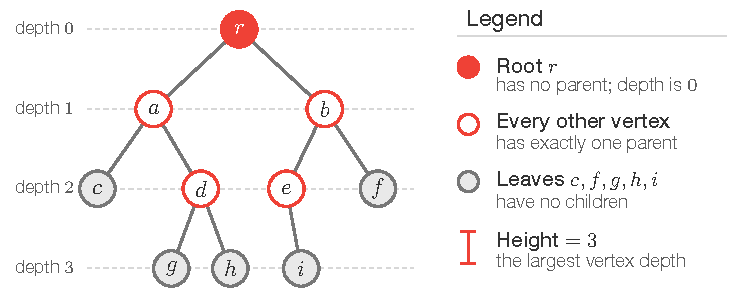
\includegraphics[height=0.58\textheight,keepaspectratio]{../figs/Fig-General-Tree-Schematic/Fig-General-Tree-Schematic-panel.pdf}
  \end{center}

  \vspace{-0.3em}
  Every non-root vertex has one parent. Vertices may have children; those with no
  children are leaves. Depth counts edges from the root, and height is the maximum depth.
\end{frame}

\begin{frame}{Spanning Trees Retain Connectivity}
  Every connected undirected graph contains a \hilite{spanning tree}: a subgraph
  with all its vertices that remains connected and has no cycles.

  \vspace{0.8em}
  \begin{itemize}\setlength{\itemsep}{0.8em}
    \item A spanning tree on $n$ vertices contains exactly $n-1$ edges.
    \item A \hilite{forest} is an undirected graph with no cycles.
    \item Each connected component of a forest is a tree.
  \end{itemize}
\end{frame}



% ==== summary ================================================
\begin{frame}{Summary}
  We described graph structure, examined three graph families, and compared
  representations for storing their connections.

  \vspace{0.7em}
  {\large\textbf{\ink{Key takeaways}}}
  \vspace{0.35em}
  \begin{itemize}\setlength{\itemsep}{0.6em}
    \item \textbf{\ink{Graph structure and measures.}} We used connectivity,
      degree, and density to describe graphs, then compared arrangements with
      the same vertex and edge counts.
    \item \textbf{\ink{Graph families.}} We related complete graphs, bipartite
      graphs, and trees to edge counts, coloring, matchings, and unique paths.
    \item \textbf{\ink{Storage and access.}} We compared edge lists, matrices,
      and adjacency lists to explain their memory use and access costs.
  \end{itemize}

  \vspace{0.5em}
  L4b turns an adjacency list into a systematic visit order; L4c uses weights
  and minimizes route cost.
\end{frame}

\transitionframe{That's a wrap. \hilite{Which graph representation would you
choose for the next algorithm, and what operation justifies that choice?}}

\end{document}
